\documentclass[fleqn]{jbook}
\usepackage{physpub}

\begin{document}

\begin{question}{$B650i(B $B1Q8l(B}{}

\begin{subquestions}
\SubQuestion
%$B<!$N#2Ld$K$D$$$F!"JL!9$N2rEzMQ;f$K2rEz$7$J$5$$(B
%$BBh#1Ld(B
$B<!$N1QJ8$rFI$_!"0J2<$N@_Ld$KEz$($J$5$$(B
\baselineskip=12pt

$B!!(BIn 1961, during the very month that President John F. Kennedy launched the race to the moon, K. Watson, B. C. Murray and H. Brown of the California Institute of Technology noted the importance of the fact that some craters in the moon's polar regions are permanently in shadow. Rather then being subjected to two weeks of blistering rays from the sun each lunar month, these sites remain eternally dark and frigid. Such ``cold traps'', they argued, might snare water dumped on the lunar surface by crashing comets or spewed forth by lunar volcanoes. And over the aeons, inky crater floors near the poles might accumulate substantial amounts of ice. Those deposits would be immensely valuable to people on future lunar bases, who could distill water from them or separate out the oxygen and hydrogen to use as rocket propellant. It took nearly three decades, but the latest robot probe, Lunar Prospector, has seemingly confirmed that frozen caches of water can indeed be found on the moon.

$B!!(BBecause none of the Apollo missions visited the moon's poles, the \underline{($B%"(B)proposal} of Watson, Murray and Brown had remained untested for 30 years. The first experimental indication came when the Department of Defense and National Aeronautics and Space Administration sent a probe called \underline{(a)Clementine} into a polar orbit around the moon in 1994.

$B!!(BClementine found evidence for ice by bouncing radar signals off the lunar surface and back to antennas on the earth. Some of the signals that were returned suggested that ice might be present near the moon's south pole. Yet Clementine uncovered no indications of ice at the north pole, even though the prove flew much lower there, and the radar experiment should have been more sensitive to ice on the surface.

$B!!(BA 1994 report by the late \underline{(b)E. M. Shoemaker and two
 colleagues} at the U.S. Geological Survey noted that the south
 pole of the moon contains ``much larger'' areas of permanent shadow
 than the north does, although just how much was hard to say. So
 Clementine's finding evidence for ice only in the south seemed to
 make some sense. But in 1997 \underline{(c)three radio
 astronomers} reported that radar reflections of the type seen by
 Clementine could also be found for sunlit parts of the moon,
 casting doubt on this earlier indication of an icy southern
 pole. \underlineeng{($B%$(B)And the latest results from Lunar Prospector
 have completely reversed the bias that had, up to this point, placed the moon's south pole in the spotlight.}

$B!!(BAccording to \underline{(d)A. B. Binder} of the Lunar Research Institute, the leader of the Lunar Prospector science team, measurements from the spacecraft show ``about twice as much water ice in the north polar regions as in the south polar regions.'' Actually, the relevant instrument on Lunar Prospector can only sense the presence of hydrogen. The conclusion that the hydrogen detected is from water, Binder admits, is \underline{($B%&(B)``a leap of faith''} but a logical one. The ice is apparently mixed with a great deal of rock, so that it makes a tiny fraction of the lunar soil. However, the ice-tinged soil may extend a couple of meters deep.

$B!!(BBinder does not yet know why the new results from Lunar Prospector show more ice in the north than in the south. He suggests that the shadow maps previously obtained from Clementine may have been misleading. Unfortunately the mystery remains unsolved for the moment: Lunar Prospector carries no camera, so the scientists cannot just take a quick look.\\
\\
snare:  $BJa$i$($k(B\\
spewed:  $B$O$-=P$5$l$k(B\\
aeons:  $B1J1s(B\\
propellant:  $B!J%m%1%C%HEy$N!K?d?J:^(B\\
caches:  $B1#$7>l(B\\
leap:  $BD7Lv(B\\

\baselineskip=15pt

\begin{subsubquestions}
\SubSubQuestion
$B2<@~It!J%"!K$N(Bproposal$B$H$O2?$+@bL@$;$h(B
\SubSubQuestion
$B2<@~It!J%$!K$rOBLu$;$h(B
\SubSubQuestion
$B2<@~It!J%&!K$K$O$I$&$$$&0UL#$,9~$a$i$l$F$$$k$+!#(B
\SubSubQuestion
$B2<@~It(B(a),(b),(c),(d)$B$K$h$k<gD%E@$J$$$74QB,7k2L$r!"$=$NAj8_4X78$,$o$+$k$h$&$KMWLs$;$h!#(B
\end{subsubquestions}

\SubQuestion
$B$D$k$^$-%P%M(B(coil spring)$B$K=E$j$r$V$i2<$2$k$H!"$=$N<+A3D9$+$i(B$x(m)$$B$@$1?-$S$k!#=E$j$,%P%M$K5Z$\$9NO(B$F(N)$$B$O!"%U%C%/$NK!B'(B(Hooke's law)$B$h$j!"(B$F=kx$$B$H=q$1$k!#$3$N;~$NHfNcDj?t(B$k(N/m)$$B$r$=$N%P%M$N%P%MDj?t(B(spring constant)$B$H$$$&!#$3$N%U%C%/$NK!B'$r3N$+$a!"%P%MDj?t(Bk$B$rB,Dj$9$k<B83$r9T$C$?!#$=$NB,Dj7k2L$O2<?^$N%0%i%U$K(B$x$$B$H(B$F$$B$N4X78$H$7$FM?$($i$l$F$$$k!#(B\\
$B$3$N<B83$rJs9p$9$k%l%]!<%H$r1QJ8$G=q$1!#$?$@$7!"(B $B#1(B.$B<B83$NL\E*!"#2(B.$B<B83J}K!!"#3(B.$B7k2L!"#4(B.$B9M;!!"#5(B.$B7kO@(B $B$N%;%/%7%g%s$O!"?t9TDxEY$N5-=R$GNI$$!#I,MW$J$i$P!"2rEzMQ;f$KE,Ev$J?^$r=q$-!"$=$l$r;2>H$7$J$,$i@bL@$7$F$b$h$$!#(B\\
\begin{center}
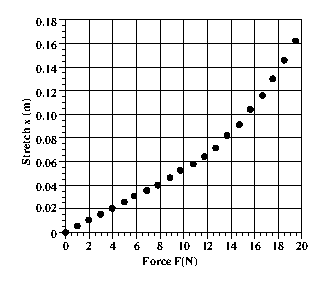
\includegraphics[clip,width=100mm]{1998eng2.eps}\\
{\Large Fig.~1}
\end{center}

\end{subquestions}
\end{question}
\begin{answer}{$B650i(B $B1Q8l(B}{}
\begin{subanswers}
\SubAnswer
  {\bf $BA4Lu(B}

$B!!(B1961$BG/(BJ.F.$B%1%M%G%#!<BgE}NN$,7n$X$N%l!<%9$r;O$a$^$7$?!#$=$N7n$K%+%k%U%)%k%K%"9)2JBg3X$N(BK.$B%o%H%=%s$H(BB.C.Murray$B!"(BH.$B%V%i%&%s$N;0?M$O$$$/$D$+$N7n$N6KCO0h$N%/%l!<%?!<$O1J5W$K1F$K$J$C$F$$$k$H$$$&;v<B$N=EMW@-$K8@5Z$7$?!#7n$N;~4V$GKh7nFs=54V!">F$1$D$/$h$&$JB@M[8w@~$K$5$i$5$l$J$$$G$3$l$i$NCO0h$O1J5W$K0E$/6K4($N$^$^$G$"$k!#H`$i$,5DO@$9$k$H$3$m$K$h$k$H!"$=$N$h$&$J!V%3!<%k%I%H%i%C%W!W$OWB@1$N>WFM$K$h$C$F7n$NI=LL$KEj$2=P$5$l$??e$d!"7n$N2P;3$NJ.$-=P$5$l$??e$rJa$i$(!"D9$$4V$N$A!"6KCOJ}$N??$C0E$J%/%l!<%?!<$NDl$K!"BgNL$NI9$r$?$a9~$s$G$$$k2DG=@-$,$"$k!#$=$NI9$OL$Mh$N7nLL4pCO$N?M$K$H$C$FHs>o$K2ACM$,$"$j!">xN1$7$F?e$rF@$?$j!";@AG$H?eAG$KJ,2r$7$F%m%1%C%H$NG3NA$K;H$C$?$j$G$-$k!#(B30$BG/6a$/7P$C$?$,!":G?7$N%m%\%C%HC5::5!!V%k%J!&%W%m%9%Z%/%?!<!W$O!"E`$C$??e$N>l=j$rK\Ev$K7n$N>e$G8+$D$1$k$3$H$,$G$-$k$H!"$&$o$Y$G$O3N$+$a$?!#(B

$B!!%"%]%m7W2h$G7n$N6KCOJ}$KK,$l$J$+$C$?$N$G!"#3?M$N0F$O#3#0G/4V<j$D$+$:$K;D$C$?!#:G=i$N<B83E*C{8u$O9qKIAm>J$H#N#A#S#A$,(B1994$BG/$K7n$N6K50F;$KAw$C$?C5::5!!"%/%l%a%s%?%$%s$rBG$A>e$2$?$H$-$KMh$?!#(B

$B!!%/%l%a%s%?%$%s$O7n$NI=LL$K%l!<%@!<$rH?<M$5$;$FI9$N>Z5r$rF@$F!"CO5e$KAw$C$F$-$?!#5"$C$F$-$??.9f$N$$$/$D$+$OI9$,Fn6K$N6a$/$K$"$k$+$bCN$l$J$$$H$$$&$3$H$r<(:6$7$F$$$?!#$7$+$7!"%/%l%a%s%?%$%s$OKL6K$G$OFn6K$h$j!"$h$jDc$/Ht$s$G$$$k$N$K$b4X$o$i$:!"2?$N>Z5r$bF@$i$l$J$+$C$?!#$=$7$F!"%l!<%@!<<B83$OI=LL>e$NI9$K$b$C$H9b46EY$K$9$kJ}$,$h$+$C$?!#(B

$B!!%"%a%j%+CO<AD4::It$N8N%7%e!<%a!<%+!<$HFs?M$NF1N=$N(B1994$BG/$NJs9p$O(B
$B$I$l$/$i$$$+$O8@$$Fq$$$,!"7n$NFn6K$NJ}$,!"KL6K$h$j$b$h$j9-$$1J5W(B
$B$N1F$r4^$`$3$H$r;XE&$7$?!#$=$&$9$k$H!"%/%l%a%s%?%$%s$,Fn6K$G$7$+(B
$BI9$N>Z5r$rF@$i$l$J$+$C$?$N$bM}$K$+$J$&$h$&$K;W$o$l$?!#$7$+$7!"(B
1997$BG/!";0?M$NEEGHE7J83X<T$OFn6K$NI9$N$3$N=i4|$N>Z5r$K5?$$$rEj$2(B
$B$+$1!"%/%l%a%s%?%$%s$K8+$i$l$?%l!<%@!<H?<M$N%?%$%W$O7n$NF|$,<M$9(B
$BItJ,$K$h$C$F$b8+$i$l$k$3$H$rJs9p$7$?!#(B\underlinejpn{$B!J%$!K$=$7$F!"7n$NC5::5!$N:G?7$N7k2L$O!"$3$N;~E@$^$G$G$OFn6K$K$OF|$,<M$9$H$$$&798~$K40A4$KLa$C$F$7$^$C$?!#(B}

$B!!!V7nC5::%A!<%`!W$N;XF3<T$G!"%k%J%j%5!<%A3X2q$N(BA.B.Binder$B$K$h$k$H!"1'ChA%$G$NB,Dj$OFn6K$h$j$bKL6K$NJ}$,FsG\$NI9$d?e$r<($7$F$$$k!#<B:]$O%k%J!&%W%m%9%Z%/%?!<$N4XO"$N$"$k7W4o$O?eAG$NB8:_$r46CN$9$k$@$1$G$"$k!#4QB,$5$l$??eAG$,?e$+$i$H$$$&7kO@$O(BBinder$B$bG'$a$F$$$k$,!"O@M}E*$J7kO@$G$J$/!"HtLv$,$"$k!#I9$OBgNL$N4d@P$H:.$6$C$F$$$k$i$7$/!"7n$NEZ$N>.$5$J$+$1$i$K$J$C$F$$$k!#$7$+$7!"I9$r4^$s$@EZ$O#2!A#3%a!<%H%k$N?<$5$^$G9-$,$C$F$$$k$@$m$&!#(B

$B!!(BBinder$B$OL$$@!V%k%J!&%W%m%9%Z%/%?!<!W$+$i$N?7$7$$>Z5r$,Fn6K$h$jKL6K$K$h$jB?$/$NI9$,$"$kM}M3$,$o$+$C$F$$$J$$!#(BBinder$B$O%/%l%a%s%?%$%s$+$iF@$i$l$?2a5n$N1F$NCO?^$,4V0c$C$F$$$k$N$G$O$J$$$+$H8@$&$3$H$rDs0F$7$F$$$k!#IT9,$J$3$H$K!":#$O$=$NFf$r2r$+$:$K;D$C$F$$$k!#%k%J!&%W%m%9%Z%/%?!<$O%+%a%i$r;}$C$F$$$+$J$+$C$?$N$G!"2J3X<T$OAGAa$/8+$k$3$H$O$G$-$J$$!#(B
\begin{subsubanswers}
\SubSubAnswer

$B7n$N6KIU6a$N%/%l!<%?!<$OB@M[$N8w$,>o$KEv$?$i$J$$$N$G!"WB@1$N>WFM$d2P;3$NJ.2P$K$h$C$F!"7n$NI=LL$K=P$??e$r!"I9$H$7$F$?$a9~$s$G$$$k2DG=@-$,$"$j!"$=$NI9$rL$Mh$N7nLL4pCO$GMxMQ$9$k$H$$$&0F!#(B

\SubSubAnswer
$BA4Lu$r;2>H(B

\SubSubAnswer
$B?eAG$NB8:_$r46CN$7$?$@$1$G!"$=$l$,?e$+$i$N$b$N$@$HH=CG$7$F$7$^$&HtLv!#(B

\SubSubAnswer
$B%/%l%a%s%?%$%s$O7n$NI=LL$+$iI9$NB8:_$r3NG'$7$?!#Fn6KIU6a$+$iI9$NH?1~$,$"$j!"KL6KIU6a$+$i$O2?$bH?1~$,$J$+$C$?!#%7%e!<%a!<%+!<C#$NJs9p$K$h$l$P!"7n$NFn6K$NJ}$,KL6K$h$j$b!"$h$j9-$$1F$,$"$k!#$=$&$9$k$H%/%l%a%s%?%$%s$N7k2L$,@5$7$$$h$&$K;W$($k!#$7$+$7!";0?M$NEEGHE7J83X<T$O%/%l%a%s%?%$%s$NF@$?I9$NH?1~$O7n$NF|$,<M$9ItJ,$+$i$b8+$i$l$k$3$H$rJs9p$7$?!#$^$?!"(BA.B.Binder$B$K$h$l$P!"%k%J!&%W%m%9%Z%/%?!<$K$h$kB,Dj$O!"Fn6K$h$j$bKL6K$NJ}$,FsG\$NI9$,$"$j!"%/%l%a%s%?%$%s$K$h$k4QB,$H$OA4$/5U$K$J$C$F$$$k!#(B
\end{subsubanswers}
\SubAnswer
$B$3$3$K$"$2$k$N$O0lNc!#(B

\begin{subsubanswers}
\SubSubAnswer
\baselineskip=12pt

\begin{itemize}
\item Purpose

I  did  an experiment with a spring in order to make sure of Hooke's law
and obtain the spring constant of it.



\parbox[t]{110mm}{
\item Procedure

Fig.~2 shows the equipment of this experiment.


I hung a \( M\)[kg] weight from the lower end of the spring and measured 
the stretch \( x\)[m] of it.



\item Results

Fig.~1(the graph in the problem paper) shows the results.


Here \( F = Mg\)[N] is the value of the force pulling the spring and
\( g\)[m/\( s^{2}\)] is the gravitational acceleration.


And the self--weight of the spring is small enough by compared with \( M\).
So it was ignored.
}
\parbox[t]{60mm}{\vspace*{3mm}
\begin{center}
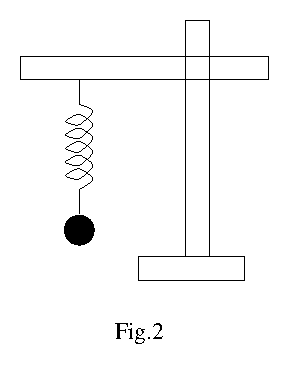
\includegraphics[clip,height=55mm,width=50mm]{1998engl.eps}
\end{center}
}

\item Consideration

From Fig.~1 when \( F\) is less than 10[N], Hooke's law is obviously valid.


But, otherwise \( F\) is not in proportion to \( x\).



\item Conclusion

A certain length \( x_{max}\) exists and \( F = kx\) (Hooke's law) is valid
for 


\( x < x_{max}\). And from Fig.~2, the spring constant \( k\)[N/m] is about 
194(for \( x \leq\) 0.06).

\end{itemize}


\SubSubAnswer

\begin{itemize}
\item The purpose of this experiment

I made sure of Hooke's law. I measured a spring constant \( k\).



\item The way of the experiment  Procedure

I hanged weight on a coil spring. I examined a relation between the
stretch \( x\) of the coilspring and the force \( F\) to pull the
coilspring.



\item The result

Fig.1 shows the relation between \( x\) and \( F\).



\item Consideration

If \( F\) is less than 12N, we find \( x\) and \( F\) follow Hooke's law.
The spring constant \( k\) is 1.8\( \times 10^{2}\)[N/m]. If \( F\) is 
stronger than 12N, \( x\) and \( F\) don't follow the law and \( F\) is
less than \( kx\).



\item Conclusion

We can conclude that if \( F\) is weak sufficiently, the coilspring follows
Hooke's law.

\end{itemize}
\SubSubAnswer

\begin{itemize}
\item Purpose

We make sure a coil spring follows Hooke's law and measure a spring constant
\( k\)[N/m].



\item Method

We hanged a weight from the coil spring and measure its stretch.



\item Result

Fig.1 shows the relationship between \( F\), which is the force given to the
coil spring and \( x\), which is the stretch of the coil spring.



\item Consideration

If \( F\) is smaller than about 12[N], the coil spring follows Hooke's law 
and the spring constant \( k\) is about 200[N/m].


If \( F\) is larger than about 12[N], \( x\) increases accelatirely and the
coil spring does not follow the hooke's law.



\item Conclusion

A coil spring follows Hooke's law when the force givn to it is small. But
if the force is large, it doesn't follow Hooke's law.

\end{itemize}

\SubSubAnswer
\begin{itemize}
\item Objective

The objective of this experiment is to confirm Hooke's law for a coil 
spring and measure the spring constant \( k\) of it.



\item Experimental Method

The stretch \( x\) of the coil spring was measured for various weights
having the different weight.



\item Result

Fig.1 provides a plot of \( x\) against the 
force \( F\) acting on the copil spring. From 
Fig.1 it can be stated that \( x\) increases 
almost linearly up to 10[N], above which it 
increases superlinearly.



\item Discussion

The result is consistent with Hooke's law up to 10[N]. Since 1/\( k\) is
equal to the slope of the fitted straight line Figure.~1, the spring constant
is 190[N/m].



\item Conclusion

\begin{itemize}
\item It is confirmed that Hooke's law is valid up to 10[N] for this coil
spring.
\item The spring constant of this spring is 190[N/m].
\end{itemize}
\end{itemize}

\baselineskip=15pt
\end{subsubanswers}

\end{subanswers}
\end{answer}


\end{document}